\chapter{Methods}
\label{methods}
\section{Protein purification} 
mEGFP or mCherry tagged tau and tau$\Delta$N, Kinesin-1, Kip3 and katanin were expressed and purified as described previously \parencite{HERNANDEZVEGA20172304,Herrmann2018,Mitra2018,NITZSCHE2010247}.

GFP-tagged, M. musculus katanin p60/p80C: katanin-GFP \parencite{Jiang2017}


\begin{figure}[h]
	\centering
	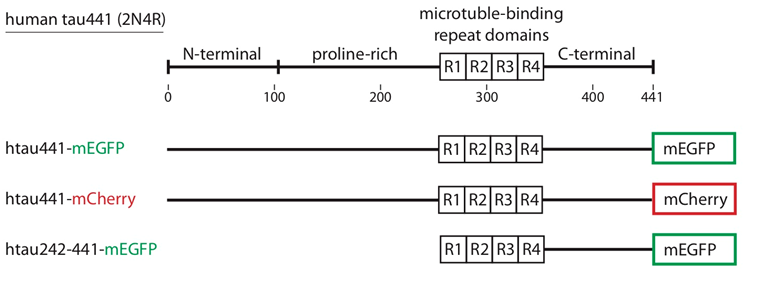
\includegraphics[width=0.6\linewidth]{Figures/tauconstructs.png}
	\caption[Schematics showing the tau constructs used in this study.]{
		Schematics showing the tau constructs used in this study.
		}\label{tauconstructs}
\end{figure}


\subsection{Microtubule preparation}
\subsection{Tubulin preparation}
Tubulin was isolated from pig brains and labeled as described previously \parencite{CASTOLDI200383}: Fresh pig brains were cleaned, homogenized in a blender in a ice-cold depolymerization buffer and centrifuged at 29.000 x g for 60 min at 4 ºC. An equal volume of high molarity PIPES supplemented with 1.5 mM ATP and 0.5 mM GTP and of 37 ºC warm glycerol was added to the supernatant to promote microtubule polymerization. The mixture was then incubated for 60 min at 37 ºC prior to centrifugation at 150.000 x g for 30 min at 37 ºC. The microtubule pellet was subsequently depolymerized by resuspension in ice-cold depolymerization buffer and dounced on ice for 10 min, followed by incubation for 60 min on ice and centrifugation at 70.000 x g for 30 min at 4 ºC. Next, the supernatant containing depolymerized tubulin was diluted in equal volumes of prewarmed high molarity PIPES and glycerol supplemented with 1.5 mM ATP and 0.5 mM GTP, incubated for 30 min at 37 ºC to promote microtubule polymerization and subsequently centrifuged at 150.000 x g for 30 min at 37 ºC. Finally, the microtubule pellet was depolymerized by resuspension in ice-cold BRB80 and dounced on ice for 10 min. After further incubation for 10 min on ice, the solution was centrifuged at 100.000 x g for 30 min at 4 ºC (SW 41Ti rotor). Tubulin was then aliquotized and flash frozen in liquid nitrogen and stored at -80 ºC for later use. Some of the tubulin was aliquotized in high concentrations for subsequent labeling as described by \cite{HYMAN1991478}. In brief, tubulin labeling involved polymerizing microtubules and incubating these microtubules with fluorescent dye present, and depolymerizing the microtubules again to yield labelled tubulin.
\subsection{Microtubule polymerization}
For preparation of biotinylated microtubules, isolated tubulin was mixed with biotinylated tubulin (Cytoskeleton Inc., T333P) at 50:1 mass ratio. For preparation of labeled microtubules, isolated tubulin was mixed with labeled tubulin. When working with microtubules, it is often desirable to stabilize microtubules, in other words, to prevent microtubule instability. We employed two techniques: i) Polymerizing microtubules under the presence of GMPCPP, a slowly hydrolyzable GTP analogue \parencite{Hyman1992}. ii) Stabilization of microtubules by having paclitaxel present in the buffer \parencite{SCHIFF1979}. GMPCPP-stabilized microtubules were grown using a mixture of 2 $\mu$M tubulin, 1 mM GMPCPP and 4 mM MgCl$_2$ in BRB80 and incubated for 3 hours at 37°C. Paclitaxel-stabilized microtubules were polymerized using a mixture of 1 mM GTP, 4 mM MgCl$_2$ and 5 \% DMSO in BRB80 for 30 minutes and subsequently stabilized by diluting the mixture in BRB80 + 10 µM paclitaxel. In both the GMPCPP and the paclitaxel procedure, the resulting mixture was then spun at 12000 g in a tabletop centrifuge. Finally, the supernatant was discarded, and the pellet was resuspended in 50 $\mu$l BRB80, respectively BRB80 + 10 µM paclitaxel. The paclitaxel-stabilized MTs were not used for assays with dynamic microtubules, as the paclitaxel would cause uninterrupted growth and inhibit catastrophes.

\subsection{Sample Preparation}
\label{assayPREP}
To conduct our microscopy, we implemented a procedure which has already been described earlier \parencite{Gell2010a}. It features TIRF microscopy of microfluidic channels which are manufactured as depicted in \autoref{Gell2010a_setup}A. The coverslips used in the process, after a cleaning procedure, were functionalized with dichlorodimethylsilane (DDS) to allow for antibody binding to the surface.\par
\begin{figure}[htb]
\centering
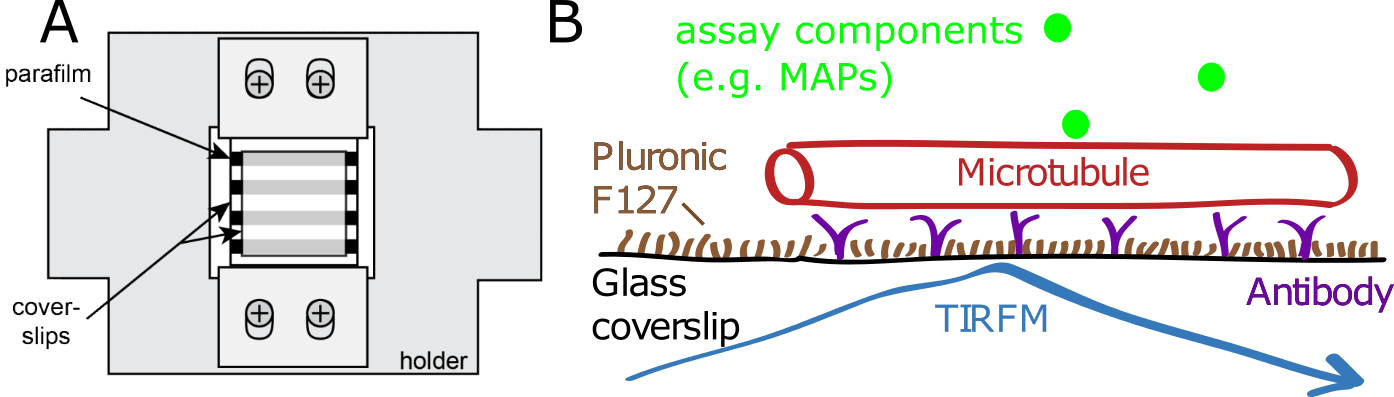
\includegraphics[scale=1.1]{Figures/setup.png}
\caption[The flow cell layout and handling, adapted from \parencite{Gell2010a}]{
		A sketch of the flow cell layout and handling, adapted from \parencite{Gell2010a}. The four depicted Parafilm stripes were put as spacers in between two DDS-coated glass slides to form three channels. To seal the channels, this construct was then heated up for about 30 seconds while gently pressing the upper slide onto the lower. Next, it was clamped into a brass sample holder. To fill the initially dry channels with liquid, vacuum was employed. Further perfusion steps were conducted by simply utilizing a filter paper as is illustrated. \textbf{B} Schematic of our our experimental setup. The labeling of our microtubules and the included assay components varied from experiment to experiment. 
	}\label{Gell2010a_setup}
\end{figure}
For some experiments (e.g. Ase1 diffusion coefficient determination), flow chambers were instead fabricated on silicon-on-insulator substrate with a diameter of around 100 mm and nominal value of the top silicon layer thickness of 50 µm based on a design prepared in Nanolithography toolbox software \parencite{Zhang2020}. Two lithography steps were performed, one defining the flow chamber, the second one for through holes. We etched the top silicon and stopped it at the buried SiO2 layer with no Si residue there, followed by anodic bonding of the silicon wafer with fabricated chambers and through holes to the corning glass type Corning 7740 with nominal thickness of 170 $\mu$m, subsequent dicing by a diamond blade dicing saw into isolated chips and coating with FAS-17 fluorosilane \parencite{Castro2018}. \par
After manufacturing, flow channels were incubated with antibodies in PBS for 1 to 5 minutes (to immobilize biotinylated microtubules, we used anti-biotin antibodies, to immobilize microtubules without biotin, we used anti-$\beta$-tubulin antibodies), followed by incubation for at least 30 min with 1\% pluronic F-127 in PBS to prevent unspecific protein binding. The flow channel was then washed with BRB80 prior to addition of microtubules for antibodyspecific binding ("template MTs"). Unbound microtubules were then removed in another wash step.\par
After these preparatory steps (and in some cases additional steps, see below sections), the assay buffer was added, the flow chambers were sealed in the case of longer experiments to prevent changes in concentrations due to evaporation, and the coverslip holder was mounted onto the microscope stage (setup shown in \autoref{Gell2010a_setup}).

\section{Imaging}
Atto647-labeled microtubules, mCherry- and mEGFP-labeled proteins were visualized sequentially by switching between the Cy5, TRITC and GFP channels (Chroma filter-cubes) using Nikon-Ti E microscope equipped with 100x Nikon TIRF objective and either Hamamatsu Orca Flash 4.0 sCMOS or Andor iXon EMCCD cameras. In the case of tau experiments, the acquisition rate varied between 1 frame per 30 ms to 1 frame per 30 seconds depending on the particular experiment and is indicated in the corresponding figure. In the case of Ase1 Set A experiments, the GFP channel was visualized or the IRM channel (or both with sequential switching), at a framerate of 5s. For Ase1 Set B experiments, channels were sequentially switched at a framerate of 2.6 seconds (with a 633x Zeiss oil immersion TIRF objective in combination with a Andor iXon DV 897 (Andor Technology) EMCCD camera). Imaging conditions in experiments used for quantitative estimation of kinetic parameters were set such that photo-bleaching effects were negligible (< 2 \% fluorescent intensity loss during the experiment). Finally, for Ase1 Set A experiments, the Alexa647-labeled MT seeds were imaged before the start of the time lapse, and only the Ase1-mNeonGreen channel was imaged during the time lapse. For set B experiments, the rhodamine (tubulin) and the GFP (Ase1-GFP) channel where imaged sequentially, whereas every 40th frame the Alexa647 channel was imaged in place of the GFP channel, in order to track the location of the GMPCPP-stabilized seeds (which we with this data determined to not move significantly during experiment time). 

\section{Image analysis}
\label{methods_analysis}
Data was analyzed using FIJI \parencite{Schindelin2012} and custom written Matlab (Mathworks) routines. 
\subsection{Density estimation}
Kymographs (KymographBuilder plugin, custom-modified to compute integrated intensity instead of finding the maximum intensity, see Zenodo: \url{doi.org/10.5281/zenodo.3270572}) along the microtubule length were used to read out the fluorescent signal and to estimate the integrated signal intensity of fluorescent proteins bound to the microtubule (if necessary, time series were drift-corrected with FIESTA \parencite{RUHNOW20112820}). The recorded signal in regions directly adjacent to the microtubule was subtracted as background signal. Kymograph pixels were then manually categorized according to the type of microtubule region they covered (island, curved microtubule, regions surrounding the islands in case of tau, overlapping microtubules or single microtubules in the case of Ase1). The integrated intensity averaged along the microtubule length for each region type was then computed by taking the mean of the categorized kymograph pixels (in the case the Ase1 assays, only regions with dynamic extensions present were measured). The density of labeled MAPs bound to the microtubule was then estimated by dividing the averaged integrated intensity by estimated intensity per single molecule times unit length. Conversion to the number of MAP molecules per tubulin dimer was performed assuming 13 available protofilaments and 8 nm length of a tubulin dimer.

\subsection{Diffusion coefficient estimation} 
Single tau molecule tracking for the estimation of diffusion coefficients (TODO, \aref{ase2FRAP}{B}) was performed using FIESTA\parencite{RUHNOW20112820} software. For reconnecting tracks, a threshold velocity of 12000 nm/s had been chosen, and tracks were allowed to have at most 3 missing frames between two data points. To minimize false-positive connecting of separate molecules, the tracks obtained by FIESTA were cut into pieces such that the maximum distance between two data points was never above 360 nm.

\subsection{Fluorescent signal of a single fluorescent molecule} 
In our assays, we often were interested in the absolute number of labeled proteins bound to microtubules. To estimate this number, it was necessary to know the contribution of single fluorophores to the measured signal. The fluorescent signal of a single fluorescent molecule was determined by generating intensity time-traces of single fluorophore-labeled kinesin-1 molecules tightly bound to the microtubule in presence of AMP-PNP (in the absence of ATP) and estimating the height of the occurring bleaching steps. The number of steps was first estimated by eye, and this number was used as input for the \textit{findchangepoints} function of Matlab to determine the position of the steps (see \autoref{bleaching_steps}). To yield the intensity per single molecule, the heights of these steps were averaged (and in the case of Ase1, multiplied by two, given that Ase1 forms homodimers).
\begin{figure}[htb]
\centering
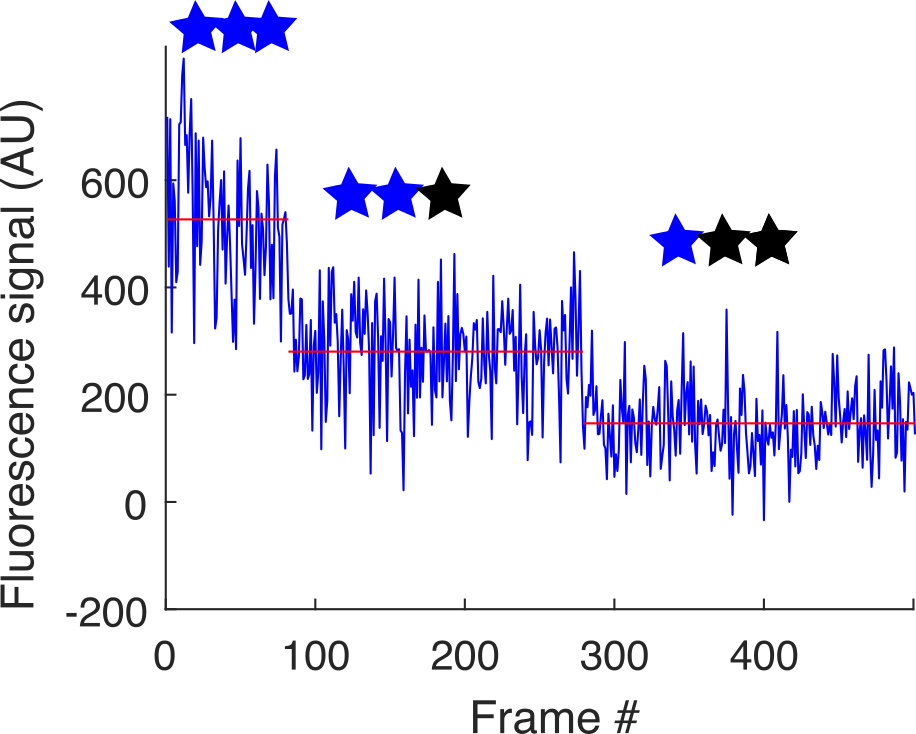
\includegraphics[scale=1.1]{Figures/bleaching_steps.png}
\caption[An illustration explaining our estimation of the fluorescent signal of a single fluorophore.]{
		The signal recorded on a particular spot on a microtubule decorated with immobilized fluorophore-labeled kinesin-1 molecules. The signal shows a step-wise decay due to photobleaching of the fluorophores. The bleaching steps were detected detection of significant changes of the mean values.
	}\label{bleaching_steps}
\end{figure}

\section{Data representation}
In all boxplots presented in the figures, horizontal midline indicates the median; bottom and top box edges indicate the 25th and 75th percentiles, respectively; the whiskers extend to the most extreme data points not considered as outliers (the function Alternative box plot from the IoSR Matlab Toolbox has been used); the numbers indicate the sample size; the notches are centered on the median and extend to ±1.58*IQR/sqrt(sample size). Where single, colored data points are presented, points from the same experiment are indicated by the same color (unless otherwise stated). 

\section{Procedures specific to tau experiments}

\subsection{Ase1 expression}
Ase1-GFP \parencite{Janson2007} and Ase1-mNeonGreen were expressed in E. coli strain BL21 (DE3) (Altium International) \alert{(the Ase1-mNeonGreen construct had been created by Lenka Grycova)}. After harvesting the cells, the cell pellet was resuspended in 5 mL ice-cold phosphate buffered saline (PBS) and stored at - 80°C for further use. For cell lysis, the cells were homogenized in 30 mL ice-cold His-Trap buffer (50 mM Na-phosphate buffer, pH 7.5, 5\% glycerol, 300 mM KCl, 1 mM MgCl2, 0.1\% tween 20, 10 mM BME, 0.1 mM ATP) supplemented with 30 mM imidazole, Protease Inhibitor Cocktail (cOmplete, EDTA free, Roche) and benzonase (Novagen) to the final concentration of 25 units/mL, then sonicated, and finally centrifuged at 45000 x g for 60 min at 4°C in the Avanti J-26S ultracentrifuge (JA-30.50Ti rotor, Beckman Coulter). The cleared cell lysate was incubated in a lysis buffer-equilibrated Ni-NTA resin (HisPur Ni-NTA Superflow Agarose, Thermo Scientific) for 2 h at 4°C. The Ni-NTA resin was sequentially washed with wash buffer I (His-Trap buffer supplemented with 60 mM imidazole), and wash buffer II (His-Trap buffer supplemented with 60 mM imidazole and 700 mM NaCl). Ase1-GFP was eluted in His-Trap buffer supplemented with 300 mM imidazole. For Ase1-mNeonGreen, after wash buffer II, the resin was washed again in wash buffer I, now supplemented with the 3C PreScisson protease (Merck Milipore), which cut Ase1-mNeonGreen off the column, at the 3C protease cleavage site positioned in between the mNeonGreen and the 6xHis-tag. The mixture was incubated over night at 4°C. Next day the beads were removed and the cleaved protein was collected. Ase1-GFP and Ase1-mNeonGreen were concentrated by spinning the sample at 3500 RPM at 4°C using a 100kDa centrifugal filter tube (Amicon Ultra-15, Merck). The second purification step for Ase1-mNeonGreen involved size exclusion chromatography, performed using a Superdex 200 10/300 column. The size exclusion buffer consisted of 100 mM Tris, 150 mM NaCl, 1 mM MgCl2, 1 mM DTT, 0.05\% Tween, 0.1 mM ATP, and 10\% glycerol. Fractions containing the protein were collected, concentrated, The final protein concentrations were measured with a NanoDrop ND-1000 spectrophotometer (Thermo Scientific) at both 280 and 506 nm absorbance. Protein was flash-frozen in liquid nitrogen and stored at -80°C. All steps in the purification were performed at 4°C.

\subsection{In vitro tau-microtubule binding assay}
Biotinylated, paclitaxel-stabilized, Atto647-labeled microtubules in BRB80T (80 mM Pipes/KOH pH 6.9, 1 mM MgCl2, 1 mM EGTA, 10 µM paclitaxel) were immobilized in a flow chamber using biotin antibodies (Sigma B3640, 20 µg/ml in PBS). Subsequently, the buffer in the flow cell was exchanged for assay buffer (20 mM HEPES pH 7.2, 1 mM EGTA, 75 mM KCl (unless stated otherwise in the main text), 2 mM MgCl2, 1 mM ATP (+Mg), 10 mM dithiothreitol, 0.02 mg/ml casein, 10 µM paclitaxel, 20 mM d-glucose, 0.22 mg/ml glucose oxidase and 20 µg/ml catalase). Then, tau in assay buffer was flushed into the flow cell at the final assay concentration stated in the main text. In experiments including multiple subsequent tau additions, the flow cell was rinsed between each tau addition by high ionic strength buffer (200 mM KCl additional to the assay buffer). To remove tau from solution during experiments presented in Figures 1 and 5, the chamber was perfused with approximately four-fold amount of the chamber volume using assay buffer not containing tau. For high concentrations of tau (>200 nM), higher volumes (up to ten-fold chamber volume) were used to remove tau. In experiments involving kinesin-8, katanin, or kinesin-1, islands were first preformed before the respective protein was added to solution (keeping the tau concentration constant). For the katanin experiment at elevated tau concentration (Figure 6) microtubules were first incubated with 0.8 µM tau-mCherry for 5 minutes. Tau-mCherry was then removed from the measurement chamber for a brief period of time (less then 1 minute) to note the position of the islands (which were obscured by the high tau-mCherry density in the island surroundings). Tau-mCherry was then again added at 0.8 µM. After 5 minutes 215 nM katanin-GFP was added to the solution (while keeping the tau concentration 0.8 µM). All experiments were performed at room temperature. 


\subsection{Coverage by tau islands}
The fraction of microtubule length covered by tau islands has been estimated by approximating islands and microtubules with segmented lines, measuring their lengths and dividing the sum of the lengths of the islands on a single microtubule (or in a field of view) by the length of the respective microtubule on which the islands were located (or by the summed length of all microtubules within a field of view).

\subsection{Estimation of velocities}
Island boundary assembly and disassembly velocities (in absence or presence of katanin or Kip3) were estimated by approximating straight lines onto segments of advancing or receding tau island edges in kymographs. The value presented in the text is a duration-weighted average of the corresponding segments. Conversion to the number of tau molecules per second was performed by multiplying this velocity by the estimated characteristic tau density within islands (in molecules per nanometer), assuming tau binding to 13 protofilaments and 8 nm length per tubulin dimer. Kip3 and kinesin-1 velocities were estimated by approximating straight lines onto kymographs of moving motors (inside/outside island). 

\subsection{Estimation of the tau unbinding time}
To estimate the unbinding times of tau from inside and outside the islands, we analyzed how the tau density in a given region decayed over time after a buffer exchange either removing tau from solution or replacing tau-mEGFP by tau-mCherry. Every analyzed region (either island or surrounding) yielded a time trace of tau density decay after a buffer exchange. Time-traces from exemplary experiments were combined to be presented in Figures \ref{tau1}F,H and \ref{tau_s1}G  such that the thick line represents the median value of all traces at the given point in time and the bounds represent the first respectively the third quartile. To estimate the mean residence times of tau inside and outside the islands, individual density time-traces as described above were fitted separately by an exponential decay using the Matlab function fit (data points taken before exchange of solution had not been taken into account). The presented fits and mean residence times have been computed by averaging the coefficients of the individual fits.

\subsection{Katanin severing rate estimation} 
Severing rates in the areas surrounding the islands were estimated by fitting exponential decay to the number of pixels in the area of the original microtubule position above a threshold value, which was manually set to encompass the microtubule. In island regions, cuts were counted. In Figure \ref{tau6}B, the estimated severing rates include both, straight and curved microtubules. In \ref{tau7}C the severing rates are sorted according to the following definition: straight microtubules were defined as microtubule stretches in which the microtubule orientation would not change beyond 10 degrees; curved regions were defined as 0.5 µm long stretches of microtubule centered at the point of highest curvature with radius < 2.5 µm.

\section{Procedures specific to Ase1 experiments}
\subsection{In vitro Ase1-microtubule binding assay}
Biotinylated, GMPCPP-stabilized, fluorescence-labeled MTs in BRB80 (80 mM Pipes/KOH pH 6.9, 1 mM MgCl2, 1 mM EGTA) were flushed into the prepared channels, were given time to bind to biotin antibodies, and were removed from solution, as described in \autoref{assayPREP}. In the case of Ase1 set B experiments, additional preparatory steps occured: First, a buffered solution with a low concentration of Ase1 was flushed in, Ase1 was allowed to sparsely bind to the template MTs, removed from solution, and subsequently non-biotinylated GMPCPP-stabilized MTs were flushed into the flow cell which got crosslinked to the template MTs by the Ase1 on these MTs. These MTs were labelled with both rhodamine and Alexa647 (represented in sketches in dark blue), while the templates in these assays were only very weakly labelled with Alexa646 (represented in sketches in light blue). Then, the "transport" MTs were removed from solution so that only transports which formed overlaps with templates would remain in the channel. \par 
The buffer in the flow cell was then exchanged for assay buffer. Finally, Ase1 in assay buffer was flushed into the flow cell at the final assay concentration stated in the main text, together with tubulin, and the channels were sealed. Set A experiments (e.g. shown in \aref{ase1a}{}) were performed at room temperature and with 32$\mu$M unlabeled tubulin present in solution. Set B experiments (e.g. shown in \aref{ase1e}{}) were performed at 29°C and with 14$\mu$M tubulin, 7\% of which was labeled with rhodamine. The following buffer components common to all used buffers in experiments involving Ase1: 20mM PIPES pH 6.9, 10mM HEPES pH 7.2, 0.5mM EGTA, 1mM MgCl2, 0.5mM Mg-ATP, 0.67mM GTP, 0.67\% Tween20, 6.7mM DTT, 0.3 mg/ml Casein, 13.5mM D-Glucose, 0.3mg/ml glucose oxidase and 0.03mg/ml catalase. The buffer for Set A experiments, in addition to these components, contained 70mM KCl, and 0.1\% Methylcellulose, 0.1\% Glycerol, 1mM sodium phosphate and 1µM ATP. The buffer for Figure Set B experiments, in addition to the components common to all buffers, contained 116mM KCl and 0.065\% Methylcellulose.

\subsection{Overlap lifetime estimation}
The lifetime of regions of microtubule overlap was estimated for two different configurations: Antiparallel “midzones”, where two dynamic extensions met and formed a dynamic “midzone” (as shown in \aref{ase1a}{left panel}), and parallel bundles of two dynamic extensions (as shown in \aref{ase1a}{right panel}). For both antiparallel midzones and parallel bundles, lifetime was taken to start upon the dynamic (GDP) lattices of each involved microtubule being crosslinked (for antiparallel configurations, we additionally required both plus ends to be within 3 microns to each other upon start of the event), and to end upon one of the involved microtubules to depolymerize back to its GMPCPP-stabilized region. Additionally, for antiparallel bundles the lifetime also ended upon the midzone ceasing to exist. If an overlapping region survived until the end of the recorded time-lapse movie, the event was registered as censored. \aref{ase1a}{A} and \aref{ase1c}{B} were generated by using the Matlab function ecdf with setting “survival”.

\subsection{Correction for Ase1 signal measurement}
For measurements of equilibrium Ase1 density, the signal per length (S) measured on isolated MTs was used to correct for the reduced illumination intensity in outer regions of the field of view, in cases where a region of interest (ROI) was located in such a region: $S_{\textrm{corrected}}(ROI) = S(ROI) * S(\textrm{isolated MT in center of field of view}) / S(\textrm{isolated MT near ROI})$.

\subsection{Determining the parameters of microtubule dynamic instability}
Parameters of MT dynamics, for set A experiments, have been estimated by generating kymographs and approximating the location of MT plus ends over time and space with straight lines (the Ase1-mNeonGreen signal was used to visually track MT ends, as MT were not imaged directly). For set B experiments, we used FIESTA to determine the locations of MTs.42 Both methods yielded polymerization and depolymerization velocities. Rescues were identified as events where a MT switches from depolymerization to polymerization before reaching the GMPCPP-stabilized seed, and catastrophes were events where polymerization was followed by depolymerization. Rescue and catastrophe frequencies were estimated by dividing the number of rescues respectively catastrophes by the sum of the total distance depolymerized respectively polymerized by all plus ends. In the case of set A experiments, we tested the 10nM only during the revision, during a time where room temperatures were less stable. Therefore, MT velocities differed from our initial experiments across all Ase1 concentrations. To be able to pool the results from these experiments with our initial results, we multiplied the velocities of these experiments by the following factor: The mean polymerization respectively depolymerization velocity of isolated MTs at 42nM of the initial experiments divided by the mean respective velocity of isolated MTs at 42nM of the experiments performed during revision (these mean velocities were weighted by the duration of each polymerization/depolymerization event). The resulting factors were 0.4 for polymerization and 0.39 for depolymerization.

\subsection{Estimation of amount of Ase1 being swept}
To estimate the number of swept Ase1 molecules for corresponding panels in \aref{ase2b}{} (Set B experiments), we first obtained density traces for each frame during a MT depolymerization period. These traces were obtained by summing the pixel intensities perpendicular to the MT, i.e., by generating kymograph where each pixel represents such a sum (\url{doi.org/10.5281/zenodo.3270572}). For each frame f we analyzed the corresponding density trace $D_f$ as follows. (1) We computed $D_s$ by subtracting the density trace $D_{before\_catastrophe}$ of the MT before the catastrophe had occurred from $D_f$ ($D_s = D_f - D_{before_catastrophe}$) (2) We obtained $x = 0 = X_{Dsmax}$, the location of the local maximum of $D_s$ in vicinity of the MT plus end. (3) We obtained $X_{Dsright}$ by finding the first local minimum of $D_s$ to the right of $X_{Dsright}$ (to reduce the effect of noise, we smoothed $D_s$ for this computation). “Right” of $D_s$, in the here-chosen coordinate system, means toward the MT seed ($x > 0$). (4) $X_{Dsleft} = X_{Dsmax} -$ 471nm (471 nm = 3 pixels). (5) We computed $D_A$. $D_A$ is equal to $D_f$ to the left of $X_{Dsmax}$, and equal to $D_s + Df(X_{Dsmax}) - D_s(X_{Dsmax})$ to the right of $X_{Dsmax}$. (6) We fitted a distribution $Y_F$ (shape see below) plus an error function $Y_E$ to $D_A$ between XDsleft and $X_{Dsright}$. We required both $Y_F$ and the error function to not have any x-offset: $Y_F$ was a right-sided decaying exponential $exp^{-x/\sigma}$ ($Y_F = 0$ where $x < 0$, and with $\lambda$ bounded between 1 and 1000 nm) convolved with a gaussian $exp^{-x2/2\sigma2}$ (with $\sigma$ bounded between 180 to 190 nm to account for the point spread function of our setup; this same $\sigma$ had been used as input for $Y_E$). Instead of a blurred right-sided decaying exponential, we for some fits (shown in \aref{ase2e}{}) used a gaussian $exp^{-x2/2\sigma_G2}$ for $Y_F$ (with a $\sigma_G$ between 180 nm and 450 nm, which was independent of the $\sigma$ used for blurring $Y_F$). We also fixed $G+E$ (plus a constant value) to approach the minimum of $D_A$ to the left of the end, and the average of $D_A$ to the right of $X_{Dsright}$ (the average of $D_A$ within 5 microns from $X_{Dsright}$, giving more weight to values close to $X_{Dsright}$). (6) We then summed the Ase1 density below $Y_F$ (as discretized in x by the pixel size), which we took as a proxy for the number of swept Ase1-GFP molecules after dividing by the intensity per Ase1 dimer (obtained as described above). 

\subsection{Fluorescence recovery after photobleaching (FRAP)}
Biotinylated GMPCPP-stabilized MTs were immobilized on the coverslip. We then flushed in the same assay buffer as for set A experiments, incubated until the Ase1 density on MTs reached a steady-state, and subsequently bleached Ase1-mNeonGreen molecules and recorded the recovering Ase1-mNeonGreen signal. We fitted the resulting recovery curve to the expression $D_s - c exp(-bt)$, where $D_s$ is the steady state density, and $c$ and $b$ are fitting parameters (see \aref{sec:FRAP}{}). Results for fitting parameter $b$ are shown in Figure S4D.

\subsection{Mathematical modelling}
The scripts to reproduce the modelling, and to plot experimental and theoretical results from \aref{ase2d}{} and \aref{ase2steady}{} can be found in Zenodo: \url{doi.org/10.5281/zenodo.12169420}. 
\subsubsection{Assumptions}
The model of Ase1 accumulation on depolymerizing MTs, and its effect on depolymerization velocity \pref{ase2d}{A} is built on the following assumptions:
\begin{enumerate}
	\item We neglect interactions between protofilaments and only consider a one-dimensional lattice, where lattice of size $a=8$nm start at index $i=1$ at the plus end, extending to $i=400$. 
	\item Only bound Ase1 molecules are considered by recording the presence or absence (0 or 1) of Ase1 in each lattice site. Bound Ase1 molecules exchange with solution with two constant rates ($k_{on},k_{off}$). Binding is only allowed if the lattice site is empty \pref{ase2d}{A}. $k_{off}$ was directly measured, and $k_{on}$ was adjusted to match the Ase1 equilibrium density on MTs \pref{ase2t1}{}.
	\item Ase1 particles on the lattice undergo unbiased diffusion characterized by a constant hopping rate ($k_h$). Hopping is only allowed to an empty site \pref{ase2d}{A}. The rate $k_h$ is calculated from the experimentally measured diffusion coefficient of Ase1 \pref{ase2t1}{}, as $k_h=D/a^2$.
	\item The Ase1 particle in the terminal site ($i=1$), cannot hop past the MT end (red arrow on the left of \aref{ase2d}{A}), but can detach with rate $k_{off}$.
	\item The terminal lattice site may dissociate from the MT, with rate $k_d$ which depends on the presence of Ase1, according to each model:
	\begin{enumerate}
		\item In Model 1, it occurs with rate $k_d^0$ if the terminal lattice site is not occupied \pref{ase2d}{B, top}, and with rate $(1-\Omega)k_d^0$ if it is occupied \pref{ase2d}{B, bottom}. $\Omega$ is a parameter between zero and one. If $\Omega=0$, the presence of Ase1 has no effect, and if $\Omega=1$, the first tubulin subunit cannot unbind if it is bound to Ase1.
		\item In Model 2, the rate of tubulin subunits loss at the plus end is reduced by a factor ($1-\Omega$) if any of the N terminal sites is occupied. At steady state, this rate is $k_d=k_0^d [1-\Omega(1-\prod_{i=1}^{i=N}(1-P_i))]$, where $P_i$ is the probability of site $i$ being occupied by Ase1.
	\end{enumerate} 
	$k_d^0$ is derived from the depolymerization rate of MTs in the absence of Ase1 ($v_0$), measured experimentally \pref{ase2t1}{}, such that  $k_d^0=v_0/a$.
	\item If the terminal lattice site dissociates when a molecule of Ase1 is bound to it, this Ase1 is lost as well \pref{ase2d}{B, bottom}.
\end{enumerate}
	
\subsubsection{Simplification to a system of constant size}
Since terminal subunits are more likely to be lost when they are without Ase1 than when they are with Ase1, any dissociation event increases the density of Ase1 remaining on the MT. This effect is only present at the MT end, and away from the end, the probability of a binding site being occupied is only determined by the binding and unbinding constants: $\alpha=k_{on}/(k_{on}+k_{off})$.
Therefore, we can restrict the model to a section of the MT with $L$ lattice sites, as long as the probability of finding a molecule at position $L$ is close to $\alpha$. When a depolymerisation event happens, we shift the lattice indexes such that site $i+1$ becomes site $i$, and set $P_{i=L}= \alpha$. 

\subsubsection{Mean field theory}
The system can be solved using a mean-field approximation, by just considering the ensemble of  $P_i$, the average probability of a site i being occupied and neglecting higher-order correlations between neighbouring sites. We can then write a set of discrete differential equations to represent the dynamics of the system:
\begin{equation}
	\frac{dP_i}{dt}=(P_{i+1}+P_{i-1}-2P_i ) k_h+(1-P_i ) k_{on}-P_i k_{off}+(P_{i+1}-P_i ) k_d
\end{equation}

Specific equations apply at the boundaries $i=1$ and $L$:
\begin{align}
	\frac{dP_1}{dt} &= k_h (P_2-P_1 )-P_1 k_{off}+(1-P_1 ) k_{on}+k_d P_2-k_d^0 P_1 (1-\Omega) \\
	dP_L/dt &= 0
\end{align}

The terms of the equation are associated with the rates of diffusion, binding, unbinding ($k_h,k_(on ),k_{off}$) which are constant, and the depolymerization rate ($k_d$), which is affected by lattice occupancy in a different way in each model (see Assumptions).\\
For Model 1, $k_d=k_d^0 (1-\Omega P_1)$.\\
For Model 2, $k_d=k_d^0 [1-\Omega+\Omega\prod_{i=1}^{i=N}(1-P_i)]$.\\
This dynamical system can be evolved from any initial conditions, converging to the unique steady-state solution for a set of given parameters. Assuming that the MT is at binding equilibrium when it starts depolymerizing, we initially set $P_i=\alpha$ for all sites. From those initial conditions, we integrate the equations numerically using Python’s \textit{odeint} function (see source code).

\subsubsection{Modelling of overlaps}
To model MT overlaps \pref{ase2d}{E,G}, we assume that the Ase1 measured in the overlaps (see Image Analysis above) is evenly distributed among 3 protofilaments that are involved in crosslinking the MTs. We neglect the other protofilaments. We had also modelled 2 protofilaments instead of 3, which did not fit the experimental data as well as 3 protofilaments.

\subsection{Comparison of experimental data and model}
To compare the predicted and observed timescale of Ase1 accumulation ($\tau$) and Ase1 accumulation at steady state ($A_{end}$), the accumulated Ase1 as a function of time was fitted to $A_{end} (1-exp^{-t/\tau})$ in experiments and model predictions (e.g., \aref{ase2d}{F} for isolated MTs at 6nM of Ase1). In the model, the accumulation of Ase1 at any given timepoint is defined as $(\sum_{i=0}^{i=L}Pi)-\alpha L$. As a proxy of velocity of depolymerization at steady state, we used the average velocity of depolymerization observed after 20 seconds of depolymerization in experiments and compared it to the depolymerization velocity at the last simulated timepoint \pref{ase2d}{F}. The 95\% confidence intervals of these magnitudes were estimated using the bootstrap method. For each experimental condition with N depolymerization events, a thousand sets of N depolymerization events were drawn through sample with replacement. For each of those sets, $\tau$ and $A_{end}$ were calculated by fitting all observations in the set, and the average velocity after 20 seconds was calculated. Then, the distribution of each magnitude across all sets was used to calculate the 95\% confidence intervals (see source code).
